\documentclass[a4paper,12pt]{scrartcl}
\usepackage[utf8]{inputenc}
\usepackage{ngerman}
\usepackage{setspace}
\onehalfspacing
\usepackage{geometry}
\usepackage{graphicx}
\geometry{a4paper, top=25mm, left=30mm, right=25mm, bottom=25mm}

\title{Proseminar 2013}
\author{Kevin Seidel \\ Studiengang Informatik \\ Matrikelnummer: 943147}

\begin{document}

\begin{titlepage}
\begin{center}
\vspace*{1.5cm}
\begin{Large}
\textbf{Universität Osnabrück} \\[1cm]
\end{Large}

\noindent\hrulefill
\\[1.5cm]
SEMINARARBEIT \\[1cm]
zum Proseminar \\[1cm]
\textbf{Makroökonomie} \\[1cm]
im Sommersemester 2013 \\[1.5cm]
Thema : \\[1cm]
\textbf{Banken und ihr systemisches Risiko} \\[1cm]
Referent: Prof. Dr. Valeriya Dinger \\[2cm]

\end{center}
\begin{flushleft}
Vorgelegt von: \hfill Kevin Seidel \\
\hfill 943147 \\
\hfill Falkenstraße 43 \\
\hfill 49124 Georgsmarienhütte
\end{flushleft}

\end{titlepage}

\newpage

\pagenumbering{Roman} 
\setcounter{page}{2}
\tableofcontents



\newpage
\pagenumbering{arabic} 
\setcounter{page}{1} 
\section{Einleitung}
Diese Seminararbeit untersucht die wissenschaftliche Arbeit ''A framework for assessing the systemic risk of major financial institutions'' von  Xia Huang, Hao Zhou und Haibin Zhu. 
Die Herren Huang, Zhou und Zhu stellen in ihrer Arbeit eine Möglichkeit vor, dass systemische Risiko anhand einer Kenngröße darzustellen, wodurch der Risikowert einfacher zu verstehen und leichter zu vergleichen ist.

Im speziellen wird von Ihnen das systemische Risiko des Finanzsektors untersucht. Dazu werden in einem Zeitraum von sieben Jahren, zwischen 2001 und 2008, die zwölf größten US-amerikanischen Finanzinstitute\footnote{Bank of America, Bank of New York, Bear Stearns, Citibank, Goldman Sachs, JP Morgan Chase, Lehman Brothers, Merrill Lynch, Morgan Stanley, State Street Corp., Wachovia und Wells Frago.} betrachtet. 
Die Frage die sie sich dabei stellten, war, wie man das systemische Risiko am Besten bestimmen und auch anschaulich darstellen kann. Eine gute Darstellung ist in sofern hilfreich, dass man durch sie auf mögliche Ausfälle der Firmen schließen kann.
Die Autoren kamen zu dem Schluss als Kenngröße für das systemische Risiko eine theoretische Versicherungsprämie zu wählen, welche die Banken in den nächsten 12 Wochen gegen Ausfälle in Höhe von 15\% oder mehr ihrer Gesamtverbindlichkeiten absichert. 

Die Besonderheiten in dieser Arbeit sind zum einen, dass die Berechnung dieser Kenngröße nicht anhand der Bilanzen, und damit quartalsweise, geschieht, sondern in sehr kurzen Zeitabständen, da auf Echtzeitdaten, wie CDS\footnote{Credit Default Swap.}-Spreads und Aktienkurse für die Berechnung zurückgegriffen wird. Des Weiteren basieren die errechneten Größen nicht auf historischen Werten, sondern sind zukunftsorientiert, da sie sich unter anderem aus den prognostizierten Ausfallwahrscheinlichkeiten und den Korrelationen der Kapitalrenditen, welche mittels der CDS-Spreads bestimmt werden, errechnen, welche ebenfalls vorwärtsgerichtet sind.

Zusätzlich dazu, untersuchen sie, wie man dieses System auf Schwachstellen durchleuchtet und diese lokalisiert. Dies ist in sofern interessant, da man sich bei bekannten Schwachstellen besser auf die möglichen Auswirkungen vorbereiten  oder diese Schwachstellen direkt eliminieren kann. 
Bei dieser Frage kommen sie zu dem Schluss, dass man die Schwachstellen am Deutlichsten mittels eines Stresstests herausstellen kann. Während dieses Stresstests wird zuerst ein Wirtschaftsmodell erstellt, auf welches dann im zweiten Schritt verschiedene Szenarien, sowohl historische als auch eigens erdachte, angewendet werden und untersucht wird, welche Auswirkungen diese Szenarien auf das Wirtschaftmodell haben. Dabei setzten sie auf ein integriertes Mikro-Makro-Modell, welches die wechselseitigen Auswirkungen zwischen dem Bankenmarkt und der restlichen Wirtschaft sehr gut abbildet.

Mittels dieses Systems kommen die Autoren zu dem Schluss, das zwischen der Korrelation der Kapitalrenditen und der Ausfallwahrscheinlichkeit ein positiver Zusammenhang besteht, was heißt, dass bei steigender Ausfallwahrscheinlichkeit die Korrelation sinkt und andersherum bei sinkendem Ausfallrisiko die Korrelation steigt. Ausserdem ist die Korrelation stark von der Fed Funds Rate\footnote{Der Zinssatz, zu welchem sich die US-amerikanischen Banken und Sparkassen untereinander Geld leihen.} und dem Term Spread\footnote{Die Differenz zwischen Langzeitzinsen und Kurzzeitzinsen.} abhängig.

Im folgenden werde ich zuerst das Vorgehen zur Bestimmung des Indikators für das systemische Risiko, in diesem Fall die theoretische Versicherungsprämie, untersuchen und darauffolgend das System des Stresstests genauer erörtern.
\newpage

\section{Bestimmung eines Indikators für das systemische Risiko}
Um eine Kenngröße für das systemische Risiko zu ermitteln, müssen zuerst die zugrundeliegenden Wert ermittelt werden. In diesem Fall setzt sich diese aus dem Risikoprofil, der prognostizierten Ausfallwahrscheinlichkeit und der Korrelation der Vermögensrenditen zusammen. Erst nachdem diese Größen ermittelt wurden, lässt sich darauf ein Indikator für das systemisches Risiko bilden.
\subsection{Ermittlung der risikoneutralen Ausfallwahrscheinlichkeiten}
Die risikoneutrale Ausfallwahrscheinlichkeit ist eine der Hauptkomponenten bei der Bestimmung des systemischen Risikos. In dieser Arbeit wird die Ausfallwahrscheinlichkeit anhand von CDS-Spreads bestimmt.

Ein Credit Default Swap ist eine Art Verischerung für Kreditgeber. Der Kreditgeber zahlt eine Vericherungsprämie, den CDS Spread, an einen Sicherungsgeber und sichert sich damit gegen diverse Ereignisse, wie Bankrott des Kreditnehmers oder Zahlungsausfälle, ab. Die Höhe der Versicherungsprämie ist abhängig von der Ausfallwahrscheinlichtkeit und dem Verlust bei Zahlungsausfall.  Tritt ein solches Ereignisse ein, zahlt der Sicherungsgeber eine Ausgleichszahlung an der Kreditgeber.

Aus den CDS Spread lässt sich nun nach Duffie (1999) und Tarashev und Zhu (2008)\footnote{vgl. Huang et al S.5.} direkt die risikoneutrale Ausfallwahrscheinlichkeit bestimmen. Für die errechnete Ausfallwahrscheinlichkeit müssen jedoch einige Vorraussetzungen erfüllt sein. Zum einen muss eine konstante und risikofreie Zinsstruktur vorliegen, zum anderen muss eine flache Terminstruktur der Ausfallintensität gegeben sein. Des Weiteren muss eine Unabhängigkeit ziwschen dem Amortisationsrisiko und dem Ausfallrisiko existieren. 

Durch die CDS Spreads können drei Faktoren für die Ausfallwarscheinlichkeit bestimmt werden. Zuerst wäre das die Kompensation von tatsächlichen Zahlungsausfällen. Hinzu kommt die Ausfallrisikoprämie, welches eine Gebühr ist, die der Kreditnehmer an den Kreditgeber zahlt, um ihn gegen mögliche, eigene Zahlungsausfälle abzusichern. Als letztes lassen sich noch weitere Prämienzahlungen aus den CDS Spreads ableiten, wie zum Beispiel die Liquiditätsrisikoprämie, eine Rendite, welche für inliquide Anleihen gezahlt wird, da ein Kauf und Verkauf für diese Art von Anleihen schwieriger ist und dieser Mehraufwand vergütet wird.

Weitere Vorteile bei der Nutzung von CDS Spreads zur Berechnung unserer Ausfallwahrscheinlichkeit ist zum einen die Risikoneutralität. Dadurch, dass bei den CDS Spreads sowohl die wirkliche Ausfallwahrscheinlichkeit, als auch die Risikoprämien berücksichtigt werden, ist es eine risikoneutrale Messung.
Ebenso ist es ein Vorteil, das die aus CDS Spreads bestimmte Ausfallwahrscheinlichtkeit zukunftsorientiert ist. Dies ist der Fall, da durch die Verwendung von CDS Spreads, die durchschnittliche risikoneutrale Ausfallwahrscheinlichkeit innerhalb der Vertragslaufzeit des Credit Default Swaps wiedergegeben wird. 
So bekommt man nicht, wie zum Beispiel durch Bilanzen, einen Blick darauf, was mit dem Unternehmen passiert ist, sondern man bekommt einen Ausblick darauf, was in nächster Zeit mit dem Unternehmen passieren wird.
Als letztes ist anzumerken, das hier die Standardannahme einer flachen Laufzeitstruktur der Ausfallintensität gemacht wird. Diese Annahme könnte in der Realität verletzt werden, dies hat jedoch keine großen Auswirkungen auf das Endergebnis.

\subsection{Korrelation der Kapitalrenditen}
Der zweite wichtige Faktor zur Ermittlung einer Kenngröße für das systemische Risiko ist die Korrelation der Zahlungsausfälle. Um diese zu bestimmen, gibt es zwei Möglichkeiten. Zum einen kann man auf historische Daten zurückgreifen und dadurch die Korrelation der Zahlungsausfälle bestimmen. Das Problem hierbei ist, das durch die Seltenheit von Zahlungsausfälle bei großen Banken kein verlässliches Ergebnis herauskommt. 

Der zweite Ansatz besagt, dass die Ausfallkorrelation indirekt berechnet wird. Dies geschieht mit Hilfe der Korrelation der Gesamtkapitalrendite vom Aktien oder Kreditmarkt. Nach Hull und White (2004) ist es in der Praxis jedoch möglich die als Stellvertreter für die Gesamtkapitalrenditenkorrelation die Korrelation des Eigenkapitals zu verwenden. Dies ist möglich, da sich aus einer Veränderung der Aktienpreise auf die Veränderung im Gesamtkapital schließen lässt.

Dieser zweite Ansatz wird auch hier genutzt, da das Eigenkapital die höchste Liquidität auf dem Markt aufweist. Der aktuelle Zustand des Marktes und das mögliche Ausfallrisiko spiegeln sich direkt in den Aktienkursen wieder. Außerdem gibt es diese Tick-by-Tick Daten nur auf dem Aktienmarkt. 
Durch diese schnellen, über kurze Zeitintervalle bestimmten Korrelationswerte ist es möglich noch bessere Vorraussagen für die zukünftigen Korrelationen zu treffen. 

Die Benutzung der Fremdkapitalkorrelation als Ersatz für die Gesamtkapitalkorrelation ist jedoch nur bei konstantem Leverage möglich, da dann gegeben ist, das die die Korrelation des Fremdkapitals gleich der Korrelation des Gesamtkapital ist. Bei zeitlich schwankendem Leverage gehen diese Werte deutlich auseinander. 
In kurzen Zeitabständen kann man jedoch davon ausgehen, dass der Leverage relativ konstant bleibt und die Abweichungen sich nicht auf das Gesamtergebnis auswirken. Deshalb werden hier nur Zeiträume, welche kürzer als ein Quartal sind, analysiert. \footnote{Ein konstanter Leverage über einen Monat war bei 11 der 12 Banken gegeben. Nach zwei Monaten waren es noch 10 Banken. Erst ab dem Zeitraum von drei Monaten war ein großer Rückgang auf 7 Banken zu beobachten. Nach 6 Monaten wiesen nurnoch 4 Banken einen konstanten Leverage vor.}


Durch diese Herangehensweise, unter der Berücksichtigung der aktuellen Marktentwicklung, statt der Analyse von historischen Daten, ist eine vorwärtsgerichtete Untersuchung der Korrelationen möglich. Das deckt sich mit unserer Berechnung der Ausfallwahrscheinlichkeiten welche ebenfalls zukunftsorientiert sind. Aus diesen beiden Tatsachen folgt, dass auch unser Indikator für das systemische Risiko ein vorwärtsgerichteter Wert und somit zukunftsorientiert ist.

\subsection{Bestimmung des Indikators für das systemische Risiko}
Nachdem die Variablen, welche zur Berechnung des systemischen Risikos benötigt werden, erfolgreich bestimmt wurden, lässt sich nur die Kenngröße für das systemische Risiko bestimmen. Die geschieht mit Hilfe der 'portfolio 'credit risk methodology''\footnote{vgl. Huang et al S.9 Z.6f.}. Durch diese Methode ist es möglich einen Indikator für das systemische Risiko unserer Banken zu erstellen. Wie schon zuvor erwähnt, handelt es sich bei diesem Indikator um die theoretische Versicherungssumme gegen Zahlungsausfälle innerhalb der nächsten 12 Monate, welche 15 Prozent oder mehr der gesamten Verbindlickeiten entsprechen.

Für die Berechnung werden die gesamten Schuldverschreibungen der Banken, gewichtet nach Höhe der Gesamtverbindlichkeiten der einzelnen Banken, in einem hypotetischen Portfolio zusammengefasst. Für dieses Portfolio wird nun die risikoneutrale Erwartung von Kreditverlusten, welche gleich oder höher einem kleinen Anteil der Gesamtverbindlichkeiten sind, errechnet.

Der Grund für die Wahl der theoretischen Versicherungssumme als Indikator gegenüber alternativen Methoden zur Bestimmung des systemischen Risikos, liegt an der einfachen Interpretation und Vergleichbarkeit dieses Werts. Dies ist möglich, da es sich bei dem Wert um eine risikoneutrale Größe handelt und nicht wie bei anderen Methoden, wie zum Beispiel der gemeinsamen Ausfallwahrscheinlichkeit oder dem erwarteten Defizit, eher um physische Größen.  
Ein weitere Grund für die Wahl ist, die Unabhängigkeit von einer Erhöhung der Gesamtverbindlichkeiten, da der Wert als Einheit pro offener Position berechnet wird.

Außerdem ist diese Indikator sehr intuitiv, da er äquivalent zu der Prämie für ein hypothetisches risikobasiertens Depositverischungsschema ist, welches alle Kreditverluste abdeckt, solange sie über dem minimalen Anteil der Gesamtverbindlichkeiten liegen.

Der Indikator für das systemische Risiko hat ebenfalls den Vorteil, dass er sich, sowohl bei einer steigenden Ausfallwahrscheinlichkeit, als auch bei steigender Korrelation, ebnefalls erhöht, was sich auch mit der generallen Annahme deckt, dass das systemische Risiko  bei höherer Fehlerrate der einzelnen Banken oder hoher Belastung eines einzelnen Risikofaktors erhöht.

Zur letztlichen Berechnung des Indikators wird eine Monte-Carlo-Simulation verwendet. Mit Hilfe dieser wird die risikoneutrale Wahrscheinlichkeit von Kreditverlusten des zugrunde liegenden Portfolios berechnet. Dafür wird nun auch der dritte Wert der Kreditrisikokomponenten mit einbezogen, der Loss Given Default oder auch Verlustquote. Dieser Loss Given Default ist unabhängig von der Ausfallwahrscheinlichkeit und folgt einer stochastischen Verteilung. Der Wert liegt zwischen 0.1 und 1 mit einem Mittel von 0.55, was sich auch mit anderen Untersuchungen deckt.

\subsection{Erstellung von Stresstest-Szenarien}
Für die Erstellung eines Stresstest Modells ist es zuerst einmal nötig die Verbindungen zwischen den makrofinanziellem Teil der Ökonomie und den Kreditrisikoparametern unseres Portfolios, den Ausfallwahrscheinlichkeiten und der Korrelation, herzustellen. Dadurch können wir später die Auswirkungen von einem Sckock auf das systemische Risiko genauer bestimmen. 
Dieser Effekt eines Schocks auf das systemische Risiko wird hier anhand von historischen Ereignissen und hypotetischen Daten untersucht. Hierfür wird ein integriertes Mikro-Makro-Modell erstellt, welches eine Verbindung zwischen den Kreditrisikofaktoren des Bankenmarktes und einer Liste von makrofinanziellen Variablen herstellt. Diese Variablen beschreiben die Entwicklungen in der Makroökonumie und auch im Finanzmarkt.
Diese Modell besteht insgesamt aus zwei Teilen. Zum einen dem Makroteil, welcher eine VAR-Analyse nutz, um den Zustand des Bankensystems unter Berücksichtigung der generellen Marktsituation, zu bestimmen. Des Weiteren liefert die Analyse auch die Rückwirkung von Veränderungen des Bankenmarktes auf den generellen Markt und stellt damit diese Verbindung dynamisch dar.

Im zweiten, dem Mikroteil, geht es um die Modellierung der Abhängigkeit des Ausfallrisikos von den Kreditrisikofaktoren des Finanzsystems und anderen Finanzmarktvariablen.



Als letztes geht es um die Erstellung eine Stresstestszenarios. Diese werden, basierend auf den hypotetischen oder historischen Schocks auf die einzelnen Variablen des genutzten VAR-Systems, erstellt. 
Dann werden diese Schocks in das dynamische Micro-Makro-System gegeben und die resultierenden Änderungen der Variablen führt dann auch zu Änderungen an der vorhergesagten Ausfallwahrscheinlichkeit und der prognostizierten Korrelation. Durch die Änderungen an diesen Kenngrößen ändert sich dann auch unser errechnetes systemisches Risiko. 

Die erste Stresstestmethode basiert auf hypothetischen Ansatz. Dabei wird das Stresstestszenario anhand von statistischen Größen der Schockvariablen in diesem Modell erstellt. Hierzu wird die Bootstrap-Methode verwendet, bei der Statistiken auf der Grundlage von Stichproben berechnet werden. Diese Methode wird angewandt, wenn die theoretische Verteilung einer Statistik nicht bekannt ist.
Das Bootstraping wird hier benutzt, um den Weg des Schocks und die Auswirkungen auf die Kreditrisikofaktoren und die makrofinanziellen Faktoren  über die nächsten 12 Wochen zu simulieren. 
Diese Simulationen sind mehrfach implementiert und die Stresstestszenarien sind definiert als Menge von Szenarien, welche eine höchst signifikante Erhöhung des systemischen Risikos zu Folge haben.
Für jede dieser Simulationen wird anschließend die Auswirkung auf den Indikator für das systemische Risiko neu berechnet. 

Die zweite Stresstestmethode nutzt historische Szenarien. Dabei werden Daten von bekannten, historischen Marktunruhen verwendet. Ein Problem das hierbei auftritt ist, dass einige Daten, wie zum Beispiel CDS Spreads und Tagesverläufe von Aktienkursen, nur über kurze Zeiträume verfügbar sind. Daher benötigt man ein angepasstes, kleineres VAR-Modell, welches nur makrofinanzielle Variablen berücksichtigt, dafür aber auch Wert über längere Zeitperioden abschätzen kann.
Der Schock auf diese makrofinanziellen Variablen wird dann in das Modell gegeben und die Auswirkungen auf die Faktoren des systemischen Risikos und auf das systemische Risiko allgemein werden beobachtet.

Diese beiden Systeme für einen Stresstest ergänzen sich gegenseitig und erzeugen ein generelles Bild über die Schwachstellen des Finanzsektors sowohl aus historischer, als auch aus statistischer Sicht. Dabei konzentrieren sich beide Methoden jedoch auf unterschiedliche Schwerpunkte.
Die erste, hypothetische Methode ist im Gegensatz zur zweiten vorrausschauend und hat den Vorteil die möglichen Bewungungen des Marktes, sowohl aufwärts als auch abwärts, genau zu beschreiben. 

Die historische Methode hingegen betrachtet nur das Rückgangsrisiko, ist jedoch leichter zu interpretieren, da man eine Verbindung zu einer historischen Krise herstellen kann. Dadurch sind die Auswirkungen und deren Ursachen leichter verständlich.
\newpage

\section{Ergebnisse unter Anwendung der Methodik}
Nun wird das vorher erläuterte Verfahren auf reale Daten angewandt, um zu überprüfen wie es sich unter echten Bedingungen verhält und ob die Ergebnisse sich mit den echten Entwicklungen decken. Dabei wird hier das Bankensystem der USA als Beispiel verwendet. Die zwölf größten Banken der USA werden dabei, als Repräsentanten für das US-Bankensystem, über die Jahre 2001 bis 2008 beobachtet. Diese Gruppe von Banken besteht aus der Bank of America, der Bank of New York, Bear Stearns, Citibank, Goldman Sachs, JP Morgan Chase, Lehman Brothers, Merrill Lynch, Morgan Stanley, State Street Corp, Wachovia und Wells Fargo. Sie wurden gewählt, da eine Veränderung des Kreditrisikos dieser Banken sich auch auf den ganzen Finanzmarkt ausüben würden.

%\begin{figure}[htb]
%	\centering
%		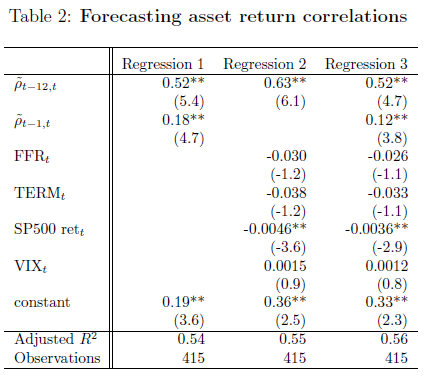
\includegraphics[height=8cm]{Pictures/Table2.png}
%		\caption{Bildunterschrift}
%\end{figure}
Dazu wird zunächst der Indikator für das systemische Risiko über die Beispielperiode bestimmt und anschließend wird mit Hilfe des Stresstests die Verwundbarkeit durch einen Schock des Systems bewertet.

\subsection{Der Indikator des systemischen Risikos}
Wie schon im vorherigen Teil, welcher auf das methodische Vorgehen eingeht, beschrieben, ist es notwendig zuerst die Ausfallwahrscheinlichkeit und die Gesamtkapitalkorrelation der Banken für den Verlauf des nächsten Quartals zu bestimmen.
Die risikoneutrale Ausfallwahrscheinlichkeit wird hier zuerst berechnet. Diese lässt sich aus den CDS Spreads ableiten und ist damit einfach zu bestimmen.
Die Korrelation lässt sich nicht von einer anderen Größe ableiten und muss daher abgeschätzt werden.


\subsubsection{Korrelationsbestimmung mit Hilfe von hochfrequenten Werten}
Um den Nutzen der Korrelationsbestimmung aus hochfrequenten Daten zu zeigen,  werden Regressionsanalysen durchgeführt. Mit Hilfe dieser Analysen ist es möglich die Beziehungen zwischen Variablen zu bestimmen.
Insgesamt sind es drei Regressionsanalysen die hier durchgeführt werden.

Für die erste Regressionsanalyse werden die erzielten Korrelationen über ein Quartal in Abständen von einer Woche verwendet. Durch den kurzen Zeitabstand von einer Woche lässt sich die zukünftige Korrelation sehr gut bestimmen, da sie auch die jüngsten Änderungen in den Korrelationen beinhalten. Das Ergebnis der Analyse zeigt, dass alle erklärenden Variablen eine starke und positive Auswirkung auf die Korrelation des nächsten Quartals haben. Die zeigt sich auch beim Bestimmtheitsmaß $R^2$ von 0.54, was auf eine starke Beziehung zwischen den Variablen hindeutet.


Die zweite Regressionsanalyse verwendet, statt der kurzzeitigen Korrelationen, eine Liste von gegenwärtigen Marktfaktoren aus der aktuellen Periode. Die verwendeten Faktoren sind zum Beispiel die Federal Funds Rate \footnote{Der Zinssatz, zu dem sich die US-amerikanischen Banken untereinander Geld leihen.}, den Term Spread \footnote{Die Differenz zwischen langfristigen und kurzfristigen Zinsen.} ,den Standard & Poor's 500 \footnote{Ein Aktienindex, welcher die 500 größten US-amerikanischen, börsennotierten Firmen umfasst.} und die implizierte Schwankungsanfälligkeit.
Die ist die beste Möglichkeit die zukünftigen Korrelationen zu bestimmen, ohne dabei auf die Tick-by-Tick Werte von Korrelationen zurückzugreifen.
Aus dieser Analyse heraus lässt sich sagen, dass man mit Hilfe der verzögerten Korrelation über ein Quartal und den Werten des Standard & Poors 500 Aktienindex, die zukünftige Korrelation gut bestimmen kann. 
Durch die Beständigkeit der Korrelation lässt sich zudem schließen, dass eine hohe verzögerte Korrelation auch zu einer hohen zukünftigen Korrelation führt und das aus niedrigen Marktgewinnen eine hohe Korrelation entsteht, welche sich  wiederum durch ein hohes systemischen Risiko ausdrückt.
Bei dieser Analyse beträgt $R^2$ = 0.55.

In der dritten Regressionsanalyse werden alle Variablen aus den hervorgegangen Analysen verwendet, was in dem Wert von 0.56 für $R^2$ resultiert. Dies zeigt, dass unter der Zuhilfenahme der verzögerten Korrelation, der Marktgewinne und hochfrequenten Korrelation, eine sehr gute Vorhersage für zukünftige Korrelationen gemacht werden kann. Dies wird noch verstärkt durch eine sehr niedrige Fehlerrate von 0.0036, welche deutlich unter der Fehlerrate liegt, die man bei einer direkten Bestimmung aus den Gesamtkapitalkorrelationen erhält (0.0051). 

\begin{figure}[htb]
	\centering
		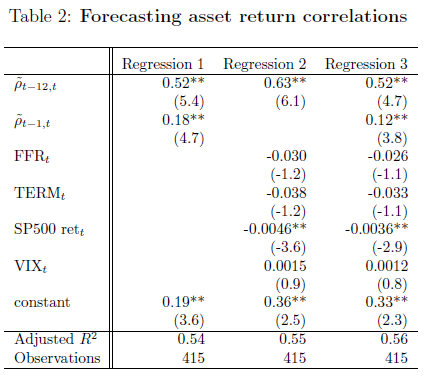
\includegraphics[height=8cm]{Pictures/Table2.png}
		\caption{Werte der Regressionsanalyse}
\end{figure}

\subsubsection{Indikator des systemischen Risikos im Bankensektor}
Durch die nun bestimmten Ausfallwahrscheinlichkeiten und Korrelation lässt sich der Indikator für das systemische Risiko gegen größere Ausfälle im Bankensektor bilden. Hier werden größere Ausfälle, als Ausfälle von mehr als 15\% der Gesamtverbindlichkeiten des Finanzsektors definiert.
Da für unsere verwendete Methodik eine risikoneutrale Ausfallwahrscheinlichkeit verwendet wird, lässt sich diese hier einfach bestimmen. Die Versicherungsprämie entspricht nämlich der Erwartung eines hypothetischen Portfolios der Banken, welche gleich gleich oder größer des Schwellenwertes von 15\% ist. Dafür die die aktuellste ''Portfolio Credit Risk Technology''\footnote{vgl. Huang et al. S.16 Z.21.} verwendet. Diese basiert auf einer Monte-Carlo-Simulation wie von Tarashev und Zhu (2008) beschrieben. 
Die Simulation besteht aus zwei Stufen. Zuerst werden verschiedene Joint Default Szenarien, basierend auf den einzelnen Ausfallwahrscheinlichkeiten und Korrelationen, simuliert. Im zweiten Schritt werden, anhand der Ergebnisse aus Schritt 1, die Loss Given Defaults und die gesamten Kreditverluste simuliert. 
Dieses Vorgehen ist zwar sehr umfangreich und mühsam, hat jedoch den Vorteil, dass es ein allgemeingültiges Ergebnis liefert.
Diese Vorgehensweise passt sehr gut zu unserer Methodik, da die Ausfallwahrscheinlichkeiten der einzelnen Banken verschiedenartig sind, die unterliegenden Variablen ungleich gewichtet sind und der Loss Given Default stochastisch unabhängig von der Ausfallwahrscheinlichkeit ist. 

\subsubsection{Verlauf des Indikators über den Beobachtungszeitraum}
Der Indikator wird hier mit Hilfe von sogenannten Basispunkten angegeben. Zum Start der Beobachtung, in der ersten Hälfte von 2001, ist der Wert des Indikators auf 10 Basispunkte festgelegt. Bis zur zweiten Hälfte von 2002 steigt der Indikator bis auf einen Wert von 35 Basispunkten, da während dieser Zeit hohe Unternehmensverluste zu beobachten waren. Nach diesem Höchststand geht der Indikator des systemischen Risikos wieder zurück, bis er zwischen Ende 2006 und Anfang 2007 seinen Tiefsstand erreicht. Erst im August 2007, zu Beginn der Immobilienkrise, ist wieder ein deutlicher Anstieg des Indikators zu beobachten. Seinen absoluten Höchststand erreichte er im März 2008, zum Höhepunkt der Immobilienkrise. Nach dem, vom Federal Reserve System \footnote{Zentralbank-System der Vereinigten Staaten von Amerika.} vereinfachtem, Aufkauf von Bear Stearn von JP Morgan Chase ging der Indikator wieder stark nach unten.

Die höchste theoretische Versicherungsprämie, die in diesem Zeitraum beobachtet wurde, war im März 2008 zu beobachten und betrug 110 Milliarden US-Dollar.
Der Trend des Indikator folgt stark dem durchschnittlichem Ausfallrisiko, wird jedoch auch noch durch die gegebenen Korrelationen beeinflusst, wenn auch nicht so stark. Der Höchstwert des Indikators fällt sowohl mit dem Maximalwert der Ausfallwahrscheinlichkeit, als auch mit dem Maximalwert der Korrelation zusammen.
Die Auswirkungen der Korrelation auf den Indikator lassen sich zum Beispiel Anfang 2001 und Anfang 2003 beobachten, wo die Ausfallwahrscheinlichkeit quasi gleich ist, der Indikator des systemischen Risikos 2003 jedoch höher ist, was mit der Korrelation zusammenhängt, welche 2003 ebenfalls höher war.

\subsubsection{Durchführung des Stresstests}
Zuerst wird der Makro-Teil des Modells durchgeführt. DIes geschieht durch eine Value at Risk-Analyse. Das Value at Risk gibt an, welchen Wert der Verlust einer Risikoposition mit einer gegeben Wahrscheinlichkeit innerhalb eines bestimmten Zeitraum nicht übersteigt. 
Die endogenen Variablen für das VAR\footnote{Value at Risk.}-Modell setzen sich aus der durschnittlichen Ausfallwahrscheinlichkeit, der Korrelation in der aktuellen Periode und einer Nummer von makrofinanziellen Faktoren zusammen. Die optimale Verzögerung innerhalb des VAR-Modells entspricht der des ''Schwart Information Criteria''\footnote{vgl. Huang et al. S.18 Z.23 S.19 Z.1.}, und zwar eine Periode. Die endogenen Variablen des Modells sind seriell korreliert, was ein starker Hinweis darauf ist, das eine dynamische Verbindung zwischen den Variablen besteht, so ist die durschnittliche Ausfallwahrscheinlichkeit stark positiv durch die durchschnittliche Korrelation beeinflusst und stark negativ von den Aktienmarktrenditen.
Daraus lässt sich nun auch herleiten, das ein höheres systemisches Risiko durch gesteigerte Korrelation zu größeren Zahlungsausfällen führt und einen Verschlechterung des Gesamtmarktes zu einer gesteigerten Ausfallwahrscheinlichkeit.
Des Weiteren lässt sich beobachten, das die durchschnittliche Korrelation stark negativ von der Federal Funds Rate und dem Term Spread beeinflusst wird, was vermuten lässt, das bei einer entspannten Geldpolitik die Kapitalrenditen der Banken enger beieinander liegen. Bei einer angespannten Geldpolitik gehen die Kapitalrenditen jedoch, abhängig vom Aufbau und Zustand der einzelnen Banken, stärker auseinander.  
Es lässt sich auch feststellen, das die Ausfallwahrscheinlichkeit einen positvien Effekt auf die Entwicklung der Korrelation hat.
Das VAR-System erlaubt es nun auch die Reaktion der Makroökonomie und des Marktes an sich auf Ereignisse des Bankensystems darzustellen. Während der Beispielperiode ist dieser Effekt jedoch nur sehr gering. Die Vermutung dahinter ist, das die durchschnittliche Ausfallwahrscheinlichkeit einen negativen Effekt auf die Federal Funds Rate hat und dadurch diesen Effekt beeinflusst.
Bei der Ausfallwahrscheinlichkeit lässt sich jedoch ein positiver Effekt auf den VIX, den Volatilitätsindex des US-Aktienindex S\&P 500, welcher die erwartete Schwankungsbreite repräsentiert, beobachten. Dies ist nachvollziehbar und verträgt sich auch mit der allgemeinen Auffassung des VIX als Maßstab der Angst des Marktes. 

Nun folgt der Mikro-Teil des Modells mit der Bestimmung der Ausfallwahrscheinlichkeiten der einzelnen Banken. Dies geschieht mit Hilfe einer Funktion von verschiedenen verzögerten und abhängigen Variablen und Variablen der aktuellen Makrtperiode, wie zum Beispiel die durchschnittliche Ausfallwahrscheinlichkeit, die Korrelation im Bankensystem und noch weiterer makrofinanzieller Faktoren.
Die Ausfallwahrscheinlichkeiten der Banken sind untereinander seriell korreliert und signifikant positiv durch die durchschnittliche Ausfallwahrscheinlichkeit des Bankensektors beeinflusst. Die Korrelationen der einzelnen Banken werden jedoch nur zu etwa der Hälfte durch die durschnittliche Korrelation auf dem Bankenmarkt beeinflusst. 

Die makrofinanziellen Faktoren wirken sich sehr unterschiedlich auf die einzelnen Banken aus. Es kann vorkommen, das sich ein Faktor kaum bis gar nicht auswirkt, es kann aber auch vorkommen das sich ein Faktor auf einige Banken positiv, auf andere widerrum negativ auswirkt. So hat die Federal Funds Rate auf vier der beobachteten Banken einen postitiven Einfluss, auf drei andere jedoch einen negativen Einfluss. Dies ist auf die unterschiedlichen Business-Modelle und Bilanzen der Banken während der Beobachtung zurückzuführen. 


Basierend auf den vorrangegangen Regressionsresultaten lässt sich der Stresstest in drei Stufen implementieren.

Zuerst werden die hypothetischen Stresstestszenarien anhand der Ergebnisse der VAR-Analysen ausgesucht.
Danach werden diese hypothetischen Szenarien in das Modell gegeben, um dann die zukünftigen dynamischen Bewegungen aller Variablen des VAR-Systems über bis zu 12 Wochen abzuleiten, da diese die zukünftigen Bewegungen der risikoneutralen Ausfallwahrscheinlichkeiten und der Korrelationen der einzelenen Banken bestimmen. 
In der letzten Stufe wird aus den Werten für die Ausfallwahrscheinlichkeit und die Korrelation, welche in der zweiten Stufe bestimmt wurden, der neue Indikator für das systemische Risiko bestimmt.


Für den wirklichen Stresstest gibt es zwei Ansätze. Einmal den statistischen und dann noch den historischen Ansatz.

Der statistische Ansatz basiert auf der Bootstraping-Methode. Dort werden die Auswirkungen eines Schocks über die nächsten 12 Monate anhand des Regressionsmodells untersucht. Als Resultat erhält man die zukünfitgen Bewegungen des Indikators für das systemische Risiko.
Bei dieser Methode war ein durschnittlicher Anstieg des Indikators auf 0.41\% zu beobachten, welcher etwa dem Niveau von Ende 2002 und Ende 2007 entspricht. In den schlechtesten 2.5\% der Szenarien stieg der Indikator auf 1.11\% und damit auf einen Wert wie im März 2008, welches dem Höchstand des Indikators entspricht. In den besten 2.5\% der Szenarien fiel der Indikator jedoch auf 0.09\%.

Der historische Ansatz basiert auf vergangenen Schocks des Systems. Hier wurden dafür zwei Beispiel-Schocks gewählt. Zum einen die ''Long Term Capital Management''-Krise von 1998, bei welcher der LTCM Hedgefonds durch falsche Spekulationen erhebliche Verluste erlitt. Zum anderen der Schock nach dem 11. September 2001.
In beiden Fällen war zu Beobachten, das der Indikator anstieg und in etwa eine Höhe wie im Januar 2008 erreichte. Er lag bei etwa 0.4\% bis 0.5\% der Gesamtverbindlichkeiten.
Die Resultate lassen vermuten, das während eines Schocks, die Anfälligkeit des Bankensystems steigt. Dies kann von einer mäßigen Anfälligkeit bis zu einer sehr starken Anfälligkeit reichen, wie es auch im Mai 2008 der Fall war. 

Der Vorteil der Bootstraping-Methode ist, dass sie die zukünfitge Verteilung der Bewegungen im systemischen Risiko simulieren kann, wodurch sie gut als Werkzeug für Vorhersagen genutzt werden kann. 


Abschließend lässt sich sagen das die Leistung des hier vorgestellten Modells sehr gut ist. Die Messungen und der Stresstest des systemischen Risikos wurden durch realen Werte bestätigt, so wurden für 375 Wochen Vorhersagen gemacht, wobei nur in 13 Wochen die Vorhersage des systemischen Risikos außerhalb des vorhergsagten Vertrauensintervalls lagen. Diese entspricht einer Fehlerquote von gerade einmal 3.5\%.
Diese Ausreißer traten auch nur bei sehr überraschenden Marktereignissen ein, so war der erste Ausreißer zwischen Juli und September 2007, zu Beginn der Immobilenkrise, zu beobachten und der zweite Ausreißer im März 2008, als die Immobilienkrise iheren Höhepunkt hatte. Diese Fehler kamen aufgrund der starken Verschlechterung des Marktes zustande, mit welcher nicht zu rechnen war.

\section{Fazit}



\begin{figure}[htb]
	\centering
		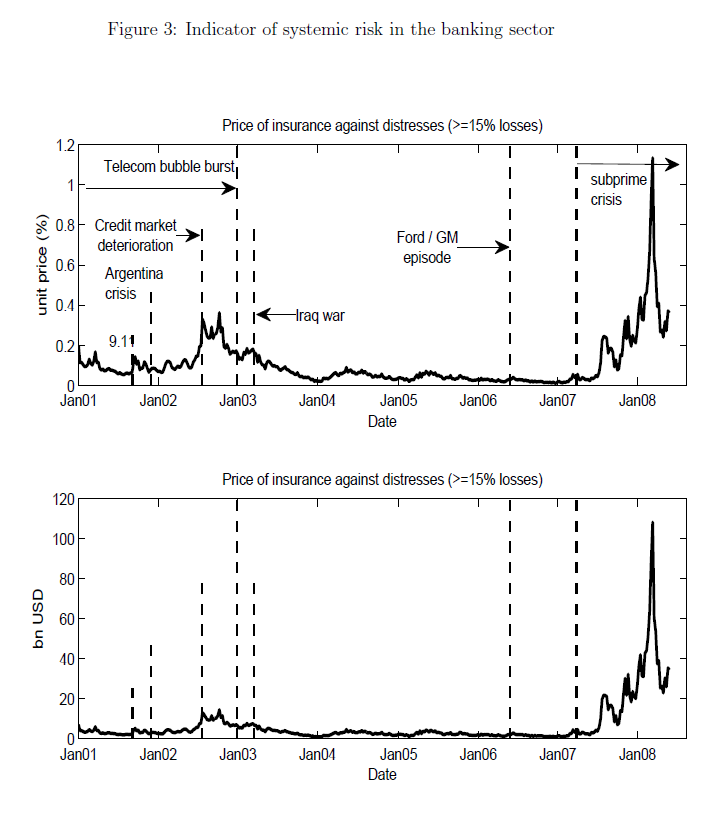
\includegraphics[height=8cm]{Pictures/Figure3.png}
		\caption{Verlauf des Indikators des systemischen Risikos}
\end{figure}


\newpage
\newpage

\section{Methodisches Vorgehen}
\subsection{Bestimmung des systemischen Risikos}
Zur Bestimmung des systemischen Risikos werden zwei Schritte durchlaufen. Zunächst wird das Risikoprofil eines Portfolios bestimmt. Dies geschieht anhand der Ausfallwahrscheinlichkeit und der Kapitalrenditen-Korrelation.
Im zweiten Schritt wird aus diesen beiden Werten der Indikator für das systemische Risiko errechnet, was in unserem Fall die Prämie einer theoretischen Versicherung gegen einen größeren Verlust ist.
\subsubsection{Risiko-neutrale Ausfallwahrscheinlichkeit}
Die Ausfallwahrscheinlichkeit beschreibt die Wahrscheinlichkeit, dass eine Forderung nicht zurückgezahlt wird.

In diesem Modell wird die risiko-neutrale Ausfallwahrscheinlichkeit verwendet. Bei einer risiko-neutralen Bewertung wird nicht wie sonst mit einem Zinssatz abgezinst, welcher eine Risikoprämie enthält, sondern mit dem risikofreien Zinssatz. Somit kann man den Erwartungswert berechnen und mit dem risikofreien Zinssatz auf den heutigen Wert abzinsen. Daraus erhält man den fairen Preis, welcher sowohl in der risikoneutralen, als auch in der nicht risikoneutralen Welt gilt.
Diese risiko-neutrale Ausfallwahrscheinlichkeit wird in unserem Fall direkt aus den Kreditausfall-Swap-Prämien errechnet. 

Die Formel hierzu lautet: 
\begin{equation}
PD_{i,t}=\frac{a_t s_{i,t}}{a_t LGD_{i,t}+b_t s_{i,t}}
\end{equation}
$PD_{i,t}$ ist hierbei die risiko-neutrale Ausfallwahrscheinlichkeit, $s_{i,t}$ ist die Kreditausfall-Swap-Prämie, $LGD_{i,t}$ ist die Verlustquote, $a_t \equiv \int_{t}^{t+T} e^{-r \tau}d \tau$ und $b_t \equiv \int_{t}^{t+T} \tau e^{-r \tau}d \tau$, wobei $r$ der risikofreie Zinssatz ist.

Das die Ausfallwahrscheinlichkeit aus den Kreditausfall-Swaps bestimmt werden, ist eine risiko-neutrale Messung, da nicht nur die Verlustwahrscheinlichkeit, sondern auch die Risikoprämie mit einbezogen wird. Des Weiteren sind die Werte vorwärtsgerichtet, denn die Kreditausfall-Swap-Prämien sind für eine bestimmte Vertragsperiode gegeben. 

Des Weiteren wird eine flache Terminstrukturkurve für die Ausfallintensität adaptiert. In der Realität könnte diese Annahme verletzt werden, es kommt aber nur zu geringer Beeinflussung, sodass das Gesamtergebnis nicht beeinträchtigt wird.
\newpage
\subsubsection{Kapitalrenditen-Korrelation}
Um die Kreditausfall-Korrelation zu bestimmen, existieren zwei mögliche Ansätze.
Zum einen kann man anhand von historischen Daten bezüglich der Kreditausfall die Korrelation bestimmen. Da es aber selten zu Kreditausfällen kommt sind diese Daten nicht sehr genau, vorallem im Bezug auf große Banken.
Die zweite Möglichkeit ist die Kreditausfall-Korrelation indirekt zu bestimmen. Dies geschieht mit Hilfe der Gesamtkapitalrenditen-Korrelation unter der Berücksichtigung des Aktien- und Kreditmarktes. Hull and White (2004) schlugen jedoch vor, die Gesamtkapitalrenditen-Korrelation durch die Fremdkapitalrenditen-Korrelation darzustellen. Dies wird in diesem Fall auch genau so umgesetzt. Die Gründe dafür sind zum einen, dass das Fremdkapital der am schnellsten gehandelte Anlagegegenstand ist, denn man sieht die Veränderungen am Markt und am Anlagerisiko direkt durch schwankende Aktienpreise. Der zweite Grund ist, dass nur auf dem Aktienmarkt Daten in Echtzeit gegeben sind, was es möglich macht, Korrelation über kurze Zeiträume zu bestimmen, was vorher, bei Verwendung von Tageswerten, nicht möglich war.
Durch diese hochfrequenten Analysen ist es nun möglich genauere Korrelationswerte als zuvor zu bestimmen.

Um statt der Gesamtkapital-Korrelation die Fremdkapital-Korrelation zu nutzen, muss gegeben sein, dass ein konstanter Leverage-Effekt vorliegt, da nur in diesem Fall die Korrelationen des Gesamt -und Fremdkapital gleich sind. Dies ist jedoch nur über kürzere Zeitabschnitte gegeben, daher werden hier die Korrelationen immer für Zeitabschnitte, welche kürzer als ein Quartal sein, bestimmt. Dieser Zeitabschnitt wurde anhand von Beobachtungen bestätigt. Nachdem bleibt im Zeitraum von einem Monat der Leverage-Effekt bei elf von zwölf Banken konstant, nach zwei Monaten sind es noch 10 von 12 und nach drei Monaten sieben von zwölf. Deshalb sollte der Beobachtungsabschnitt unter einem Quartal liegen.

Durch die Nutzung von Vorhersagen der Kapitalrenditen-Korrelation, statt dem Heranziehen von historischen Werten, sind die Werte konsistent mit der Vorhersage der Ausfallwahrscheinlichkeiten. Dadurch ist unser Indikator für das systemische Risiko vorwärtsgerichtet. 

\newpage
\subsection{Stresstest}

Blabla!
\newpage
\section{Daten}
Für die empirische Überprüfung der vorher beschriebenen Methoden werden Messwerte benötigt. Hier werden Werte aus dem Bankwesen benutzt, prinzipiell lassen sich mit dieser Methodik aber auch andere Portfolios untersuchen, solange sie die benötigten Vorraussetzungen, wie z.B. einen Kreditausfall-Swap, besitzen. 
Die hier verwendeten Messwerte stammen aus dem Zeitraum von Januar 2000 bis zum Mai 2008. Es wurden die, zu der Zeit, größten amerikanischen Finanzunternehmen untersucht. Zu den gehörten die Bank of America, Bank of New York, Bear Stearns, Citibank, Goldman Sachs, JP Morgan Chase, Lehman Brothers, Merrill Lynch, Morgan Stanley, State Street Corp, Wachovia und Wells Fargo. 
Für die Analysen wurden wöchentlich aktualisierte Kreditausfall-Swap-Prämien, Korrelationswerte, welche aus den täglichen Aktienkursen errechnet wurden, und makro-finanzielle Werte, die den aktuellen Zustand der Makroökonomie wiederspiegeln,  verwendet.

\newpage
\section{Empirisches Ergebnis}
\newpage
\section{Fazit}
\newpage
\section{Literaturverzeichnis}

Duffie, D., 1999. Credit swap valuation. Financial Analysts Journal 55, 73-87.

Tarashev, N., Zhu, H., 2008. The pricing of portfolio credit risk: Evidence from the credit derivatives Market. Journal of Fixed Income 18, 5-24.
\newpage

\section{Anhang}


\end{document}